\documentclass{article}

\usepackage{geometry}
\usepackage{amsmath}
\usepackage{graphicx}
\usepackage{listings}
\usepackage{hyperref}
\usepackage{multicol}
\usepackage{fancyhdr}
\pagestyle{fancy}
\hypersetup{ colorlinks=true, linkcolor=black, filecolor=magenta, urlcolor=cyan}
\geometry{ a4paper, total={170mm,257mm}, top=20mm, right=20mm, bottom=20mm, left=20mm}
\setlength{\parindent}{0pt}
\setlength{\parskip}{1em}
\renewcommand{\headrulewidth}{0pt}
\lhead{Competitive Programming - Arkavidia V}
\fancyfoot[CE,CO]{\thepage}
\lstset{
    basicstyle=\ttfamily\small,
    columns=fixed,
    extendedchars=true,
    breaklines=true,
    tabsize=2,
    prebreak=\raisebox{0ex}[0ex][0ex]{\ensuremath{\hookleftarrow}},
    frame=none,
    showtabs=false,
    showspaces=false,
    showstringspaces=false,
    prebreak={},
    keywordstyle=\color[rgb]{0.627,0.126,0.941},
    commentstyle=\color[rgb]{0.133,0.545,0.133},
    stringstyle=\color[rgb]{01,0,0},
    captionpos=t,
    escapeinside={(\%}{\%)}
}

\begin{document}

\begin{center}
    \section*{I. Investasi Restoran}

    \begin{tabular}{ | c c | }
        \hline
        Batas Waktu  & 1s \\
        Batas Memori & 512MB \\
        \hline
    \end{tabular}
\end{center}

\subsection*{Deskripsi}

Arvy akhirnya keluar dari perusahaan teknologinya untuk menjadi seorang wiraswasta.
Ia ingin menginvestasikan sisa gajinya untuk membangun restoran canggih yang menggunakan \textit{conveyor belt} untuk menyajikan makanan.

\begin{center}
    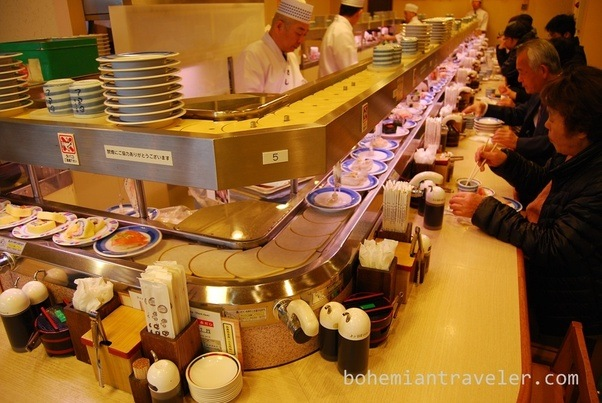
\includegraphics[width=180px]{conveyor-belt}

    \footnotesize Sumber: \href{https://www.quora.com/How-much-food-should-I-take-at-a-conveyor-belt-sushi-restaurant-I-am-an-exchange-student-in-Japan-and-my-host-family-is-taking-me-to-a-restaurant-where-you-take-all-you-can-eat-How-much-should-I-take-The-family-seems-fairly-well-off}{quora.com}
\end{center}

\textit{Conveyor belt} adalah lintasan siklik terdiri dari $N$ bagian yang dinomori dari $1$ hingga $N$.
Tiap bagian berisi maksimal 1 makanan.
\textit{Conveyor belt} akan terus bergeser sejauh 1 bagian tiap detiknya.
Dengan kata lain, apabila pelanggan ada di depan bagian nomor $X$, maka 1 detik kemudian ia ada di depan $X + 1$ (atau $1$ jika $X = N$).
Pelanggan dapat memesan beberapa makanan pada restoran tersebut dan makanan akan diletakkan pada bagian-bagian pada \textit{conveyor belt}.

Tiap makanan dimakan dengan durasi yang sama, yaitu $P$ detik.
Pelanggan pada awalnya duduk di depan suatu bagian \textit{conveyor belt} dan menunggu hingga di depannya terdapat makanan.
Jika ia sudah berhadapan dengan sebuah makanan, ia akan segera memakannya.
Setelah makanan dihabiskan, pelanggan akan kembali menunggu hingga makanan selanjutnya ada di depannya untuk dihabiskan.
Pelanggan tidak akan berpindah tempat hingga semua makanannya habis.

Bantulah Arvy memberi saran pada para pelanggan untuk menentukan posisi duduk awal agar waktu durasi makan semua makanan menjadi sesedikit mungkin.

\subsection*{Format Masukan}

Baris pertama terdiri dari satu bilangan bulat positif $T$ ($1 \leq T \leq 10$), menyatakan banyaknya kasus uji.

Tiap kasus uji diawali dengan 3 buah bilangan, yaitu $N$ ($1 \leq N \leq 200$) yang menyatakan panjang \textit{conveyor belt}, $M$ ($1 \leq M \leq N$) yang menyatakan banyaknya makanan yang dipesan, dan $P$ ($1 \leq P \leq 1.000.000.000$) yang menyatakan waktu yang dibutuhkan untuk memakan 1 makanan.

Baris berikutnya terdiri $M$ bilangan berbeda, dengan bilangan ke-$i$ adalah $A_i$ ($1 \leq A_i \leq N$), menyatakan posisi makanan ke-$i$ pada \textit{conveyor belt}.

\subsection*{Format Keluaran}

Untuk tiap kasus uji, tuliskan 1 baris yang terdiri dari 2 buah bilangan.
Bilangan pertama merupakan posisi awal pelanggan harus ditempatkan.
Bilangan kedua menyatakan waktu minimal pelanggan berada pada restoran tersebut.
Jika ada beberapa posisi awal yang mungkin, keluarkan posisi awal di bagian dengan nomor paling kecil.
\\

\begin{multicols}{2}
\subsection*{Contoh Masukan}
\begin{lstlisting}
1
7 3 3
1 4 2
\end{lstlisting}
\columnbreak
\subsection*{Contoh Keluaran}
\begin{lstlisting}
1 11
\end{lstlisting}
\vfill
\null
\end{multicols}

\subsection*{Penjelasan}
Berikut adalah simulasi pemilihan tempat optimal, yaitu posisi nomor 1:

\begin{enumerate}
    \setlength{\itemsep}{0pt}
    \item Pada detik ke-0, berada di depan bagian nomor 1, ambil makanan
    \item Pada detik ke-3, berada di depan bagian nomor 4, terdapat makanan dan bisa langsung diambil
    \item Pada detik ke-6, berada di depan bagian nomor 7, tunggu hingga ada makanan
    \item Pada detik ke-8, berada di depan bagian nomor 2, terdapat makanan dan bisa diambil
    \item Pada detik ke-11, semua makanan telah habis
\end{enumerate}

\pagebreak

\end{document}
